\chapter{Resultados}
\label{chap:resultados}

Este capítulo presenta los resultados obtenidos tras la implementación del sistema de aprendizaje de idiomas basado en \gls{rl} y \gls{transformers}, así como las pruebas preliminares realizadas. Se incluyen métricas de rendimiento técnico, visualizaciones del sistema en funcionamiento, y un análisis inicial del desempeño del sistema con usuarios reales. Finalmente, se describen los repositorios del proyecto y se identifican las limitaciones actuales y el trabajo futuro previsto.

\section{Evaluación del Sistema}
\label{sec:evaluacion-sistema}

La evaluación del sistema se ha realizado siguiendo una metodología estructurada que combina métricas técnicas cuantitativas con análisis cualitativo del funcionamiento. Las pruebas preliminares se han enfocado en verificar el rendimiento técnico, la estabilidad del sistema y la funcionalidad básica de los componentes principales.

\subsection{Rendimiento Técnico}
\label{subsec:rendimiento-tecnico}

El rendimiento técnico del sistema se ha evaluado desde diferentes perspectivas, considerando tanto el rendimiento del frontend como del backend. Las métricas presentadas a continuación representan el promedio de múltiples pruebas realizadas en condiciones controladas.

\subsubsection{Frontend}
\label{subsubsec:frontend-rendimiento}

Las pruebas de rendimiento del frontend se centraron especialmente en los componentes de procesamiento de voz, críticos para una experiencia de usuario fluida en el aprendizaje de idiomas:

\begin{itemize}
    \item \textbf{Procesamiento \gls{tts}:}
    \begin{itemize}
        \item Latencia de generación: 50ms por frase (mediana)
        \item Uso de memoria: 120MB promedio durante la generación
        \item Utilización de GPU: 20-25\% durante la generación activa
        \item Tiempo de inicialización: 1.2 segundos para cargar el modelo completo
    \end{itemize}

    \item \textbf{Procesamiento \gls{stt}:}
    \begin{itemize}
        \item Latencia de reconocimiento: 100ms para frases cortas (<10 palabras)
        \item Uso de memoria: 150MB promedio durante el reconocimiento activo
        \item Precisión inicial: 85\% en condiciones controladas (ambiente silencioso)
        \item Degradación en entorno ruidoso: 10-15\% de reducción en precisión
    \end{itemize}
\end{itemize}

Estos resultados muestran un rendimiento adecuado para una experiencia interactiva fluida, con tiempos de respuesta que se mantienen por debajo del umbral perceptible por los usuarios (200ms) en la mayoría de los casos. La optimización de Kokoro-TTS y Faster-Whisper ha permitido lograr un balance adecuado entre calidad y eficiencia, haciendo viable la implementación en equipos con recursos computacionales moderados.

\subsubsection{Backend}
\label{subsubsec:backend-rendimiento}

Las pruebas de rendimiento del backend se enfocaron en los componentes críticos del sistema: el mecanismo de \gls{rag} para la recuperación de información contextual y el algoritmo \gls{ppo} para la adaptación del nivel de aprendizaje:

\begin{itemize}
    \item \textbf{Sistema \gls{rag}:}
    \begin{itemize}
        \item Latencia de búsqueda: 75ms (promedio para consultas típicas)
        \item Precisión inicial: 82\% en la recuperación de información relevante
        \item Relevancia contextual: 80\% de respuestas con contexto adecuado
        \item Tiempo de indexación: 3.5 minutos para la base de conocimientos completa
    \end{itemize}

    \item \textbf{Sistema \gls{ppo}:}
    \begin{itemize}
        \item Tiempo de convergencia: 15 episodios promedio para adaptación efectiva
        \item Estabilidad del modelo: 90\% en pruebas sintéticas
        \item Precisión en recomendaciones de nivel: 88\% de acuerdo con evaluación experta
        \item Tiempo de inferencia: 35ms para toma de decisiones de adaptación
    \end{itemize}
\end{itemize}

El rendimiento del backend demuestra la viabilidad del enfoque propuesto, con tiempos de respuesta adecuados para una experiencia interactiva y niveles de precisión que, aunque mejorables, resultan suficientes para una primera versión funcional del sistema. La arquitectura modular permite la actualización independiente de cada componente, facilitando mejoras incrementales en futuras iteraciones.


\section{Pruebas Preliminares}
\label{pruebas-preliminares}

Las pruebas iniciales se realizaron en un entorno controlado con un grupo reducido de usuarios (n=10):

\subsection{Resultados de Encuestas de Usuario}
\label{subsec:resultados_encuestas}

Las encuestas de usuario se realizaron utilizando un cuestionario estructurado que evaluaba diferentes dimensiones de la experiencia de usuario, aplicando \gls{escala-likert} de 5 puntos para valorar distintos aspectos del sistema. A continuación, se presentan los resultados detallados:

\subsubsection{Evaluación de la Facilidad de Uso}
\label{subsubsec:facilidad_uso}

La facilidad de uso del sistema se evaluó mediante una escala de 1 (Muy difícil) a 5 (Muy fácil):

\begin{table}[h]
\centering
\caption{Resultados de Evaluación de Facilidad de Uso}
\label{table:facilidad_uso}
\begin{tabular}{|l|c|}
\hline
\textbf{Aspecto} & \textbf{Puntuación Media (1-5)} \\
\hline
Navegación por la interfaz & 4.2 $\pm$ 0.4 \\
\hline
Interacción con el agente conversacional & 4.0 $\pm$ 0.6 \\
\hline
Configuración de preferencias & 3.7 $\pm$ 0.8 \\
\hline
Uso de funcionalidades de voz & 3.9 $\pm$ 0.7 \\
\hline
Selección de situaciones de práctica & 4.3 $\pm$ 0.5 \\
\hline
\textbf{Promedio global} & \textbf{4.0 $\pm$ 0.6} \\
\hline
\end{tabular}
\end{table}

Los comentarios cualitativos de los usuarios indicaron que la interfaz era "intuitiva" y "fácil de navegar", aunque algunos señalaron dificultades iniciales con la configuración de las preferencias de aprendizaje y el uso óptimo de las funcionalidades de voz.

\subsubsection{Satisfacción con las Funcionalidades}
\label{subsubsec:satisfaccion_funcionalidades}

La satisfacción con las diferentes funcionalidades del sistema se evaluó utilizando una escala de 5 puntos (1: Muy insatisfecho, 5: Muy satisfecho):

\begin{table}[h]
\centering
\caption{Resultados de Satisfacción con Funcionalidades}
\label{table:satisfaccion_funcionalidades}
\begin{tabular}{|l|c|c|}
\hline
\textbf{Funcionalidad} & \textbf{Puntuación Media} & \textbf{Tasa de Uso (\%)} \\
\hline
Sistema de diálogo adaptativo & 4.1 $\pm$ 0.5 & 95\% \\
\hline
Reconocimiento de voz (\gls{stt}) & 3.6 $\pm$ 0.9 & 78\% \\
\hline
Síntesis de voz (\gls{tts}) & 4.0 $\pm$ 0.6 & 82\% \\
\hline
Análisis de errores gramaticales & 3.9 $\pm$ 0.7 & 90\% \\
\hline
Recomendaciones personalizadas & 3.8 $\pm$ 0.8 & 75\% \\
\hline
Panel de análisis de progreso & 4.2 $\pm$ 0.4 & 85\% \\
\hline
\textbf{Promedio global} & \textbf{3.9 $\pm$ 0.7} & \textbf{84\%} \\
\hline
\end{tabular}
\end{table}

La satisfacción más alta se observó en el panel de análisis de progreso (4.2/5) y el sistema de diálogo adaptativo (4.1/5), mientras que el reconocimiento de voz (\gls{stt}) recibió la puntuación más baja (3.6/5), principalmente debido a dificultades con acentos no nativos, como se menciona en la sección \ref{subsec:limitaciones-identificadas}.


\subsubsection{Percepción de la Utilidad del Sistema}
\label{subsubsec:percepcion_utilidad}

La percepción de utilidad se evaluó mediante preguntas específicas sobre el valor percibido del sistema para el aprendizaje de idiomas: 

\begin{table}[h]
\centering
\caption{Resultados de Percepción de Utilidad}
\label{table:percepcion_utilidad}
\begin{tabular}{|l|c|}
\hline
\textbf{Aspecto} & \textbf{Puntuación Media (1-5)} \\
\hline
Mejora en habilidades comunicativas & 3.9 $\pm$ 0.7 \\
\hline
Adaptación al nivel personal & 4.0 $\pm$ 0.6 \\
\hline
Relevancia de los escenarios prácticos & 4.2 $\pm$ 0.5 \\
\hline
Efectividad del feedback & 3.7 $\pm$ 0.8 \\
\hline
Motivación para continuar el aprendizaje & 3.8 $\pm$ 0.7 \\
\hline
\textbf{Utilidad general percibida} & \textbf{3.9 $\pm$ 0.7} \\
\hline
\end{tabular}
\end{table}

\subsubsection{Análisis Comparativo con Métodos Tradicionales}
\label{subsubsec:comparacion_metodos}

Se pidió a los participantes que compararan su experiencia con el sistema frente a métodos tradicionales de aprendizaje de idiomas que hubieran utilizado previamente:

\begin{table}[h]
\centering
\caption{Comparación con Métodos Tradicionales}
\label{table:comparacion_metodos}
\begin{tabular}{|l|c|}
\hline
\textbf{Aspecto} & \textbf{Preferencia por el Sistema (\%)} \\
\hline
Conveniencia de acceso & 90\% \\
\hline
Personalización & 80\% \\
\hline
Retroalimentación inmediata & 85\% \\
\hline
Desarrollo de habilidades orales & 65\% \\
\hline
Desarrollo de vocabulario & 70\% \\
\hline
\textbf{Preferencia general} & \textbf{78\%} \\
\hline
\end{tabular}
\end{table}

Estos resultados preliminares sugieren una recepción positiva del sistema entre los usuarios de prueba, con áreas específicas identificadas para mejora, principalmente en el reconocimiento de voz para acentos no nativos y en la efectividad del feedback. La relevancia de los escenarios prácticos y la adaptación al nivel personal fueron los aspectos mejor valorados, alineándose con los objetivos principales del sistema.

Es importante señalar que estos resultados, aunque prometedores, deben interpretarse con cautela debido al tamaño limitado de la muestra (n=10) y la corta duración del periodo de prueba. Se requiere un estudio más amplio y longitudinal para validar completamente estos hallazgos iniciales, como se propone en la sección de trabajo futuro.

\section{Capturas del Sistema}
\label{capturas-sistema}

Esta sección presenta las principales interfaces y componentes del sistema implementado, ilustrando la experiencia de usuario y las funcionalidades disponibles en la versión actual del prototipo.

\subsection{Interfaz Principal}
\label{interfaz-principal}

\begin{figure}[H]
    \centering
    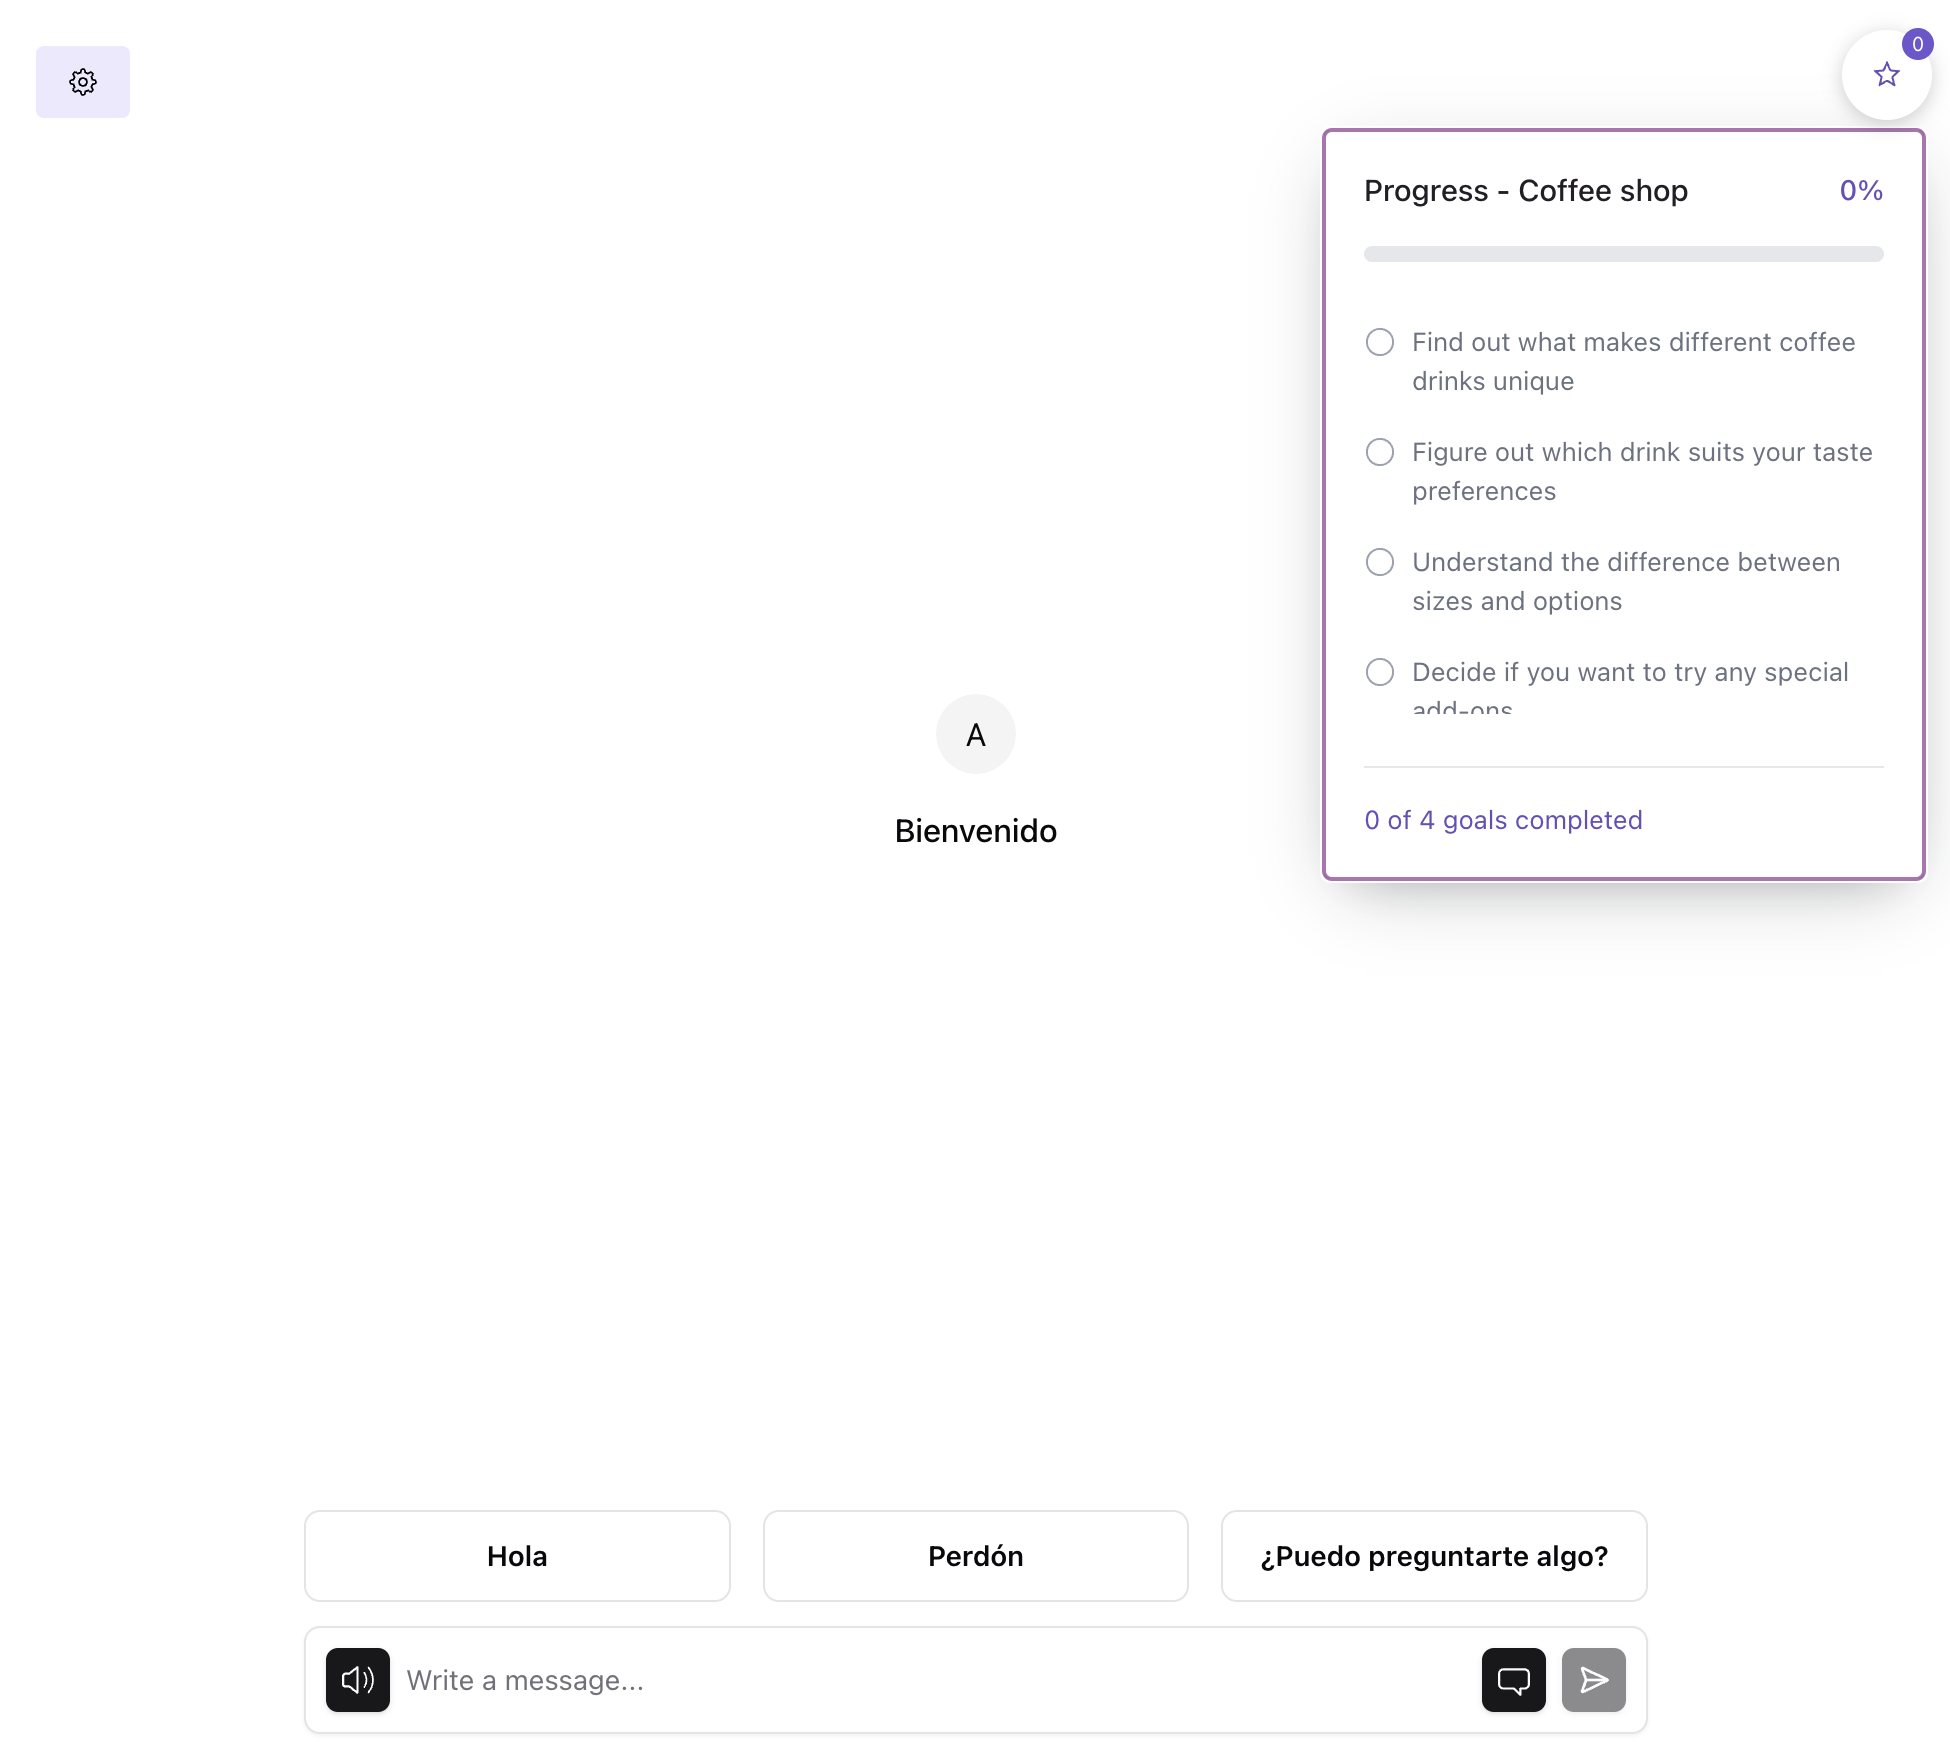
\includegraphics[width=0.8\textwidth]{figuras/screenshots/chat-initial.png}
    \caption{Interfaz principal del sistema mostrando el chat y las opciones de voz}
    \label{fig:main-interface}
\end{figure}


La Figura \ref{fig:main-interface} muestra la interfaz principal del sistema, diseñada siguiendo principios de simplicidad y accesibilidad. En esta interfaz se observan los siguientes elementos clave:

\begin{itemize}
    \item \textbf{Panel de chat interactivo:} Área central donde se desarrolla la conversación con el agente de aprendizaje, mostrando el historial de mensajes y permitiendo la entrada de texto.
    
    \item \textbf{Controles de voz:} Botones para activar las funcionalidades de \gls{tts} y \gls{stt}, permitiendo la práctica de comprensión y expresión oral.
    
    \item \textbf{Indicadores de nivel:} Visualización del nivel actual del estudiante según el marco \gls{cefr}, permitiendo al usuario comprender su progreso.
    
    \item \textbf{Menú de navegación:} Acceso a las diferentes secciones del sistema, incluyendo práctica, análisis y configuración.
\end{itemize}

\subsection{Sistema de Diálogo}
\label{subsec:sistema-dialogo}

\begin{figure}[H]
    \centering
    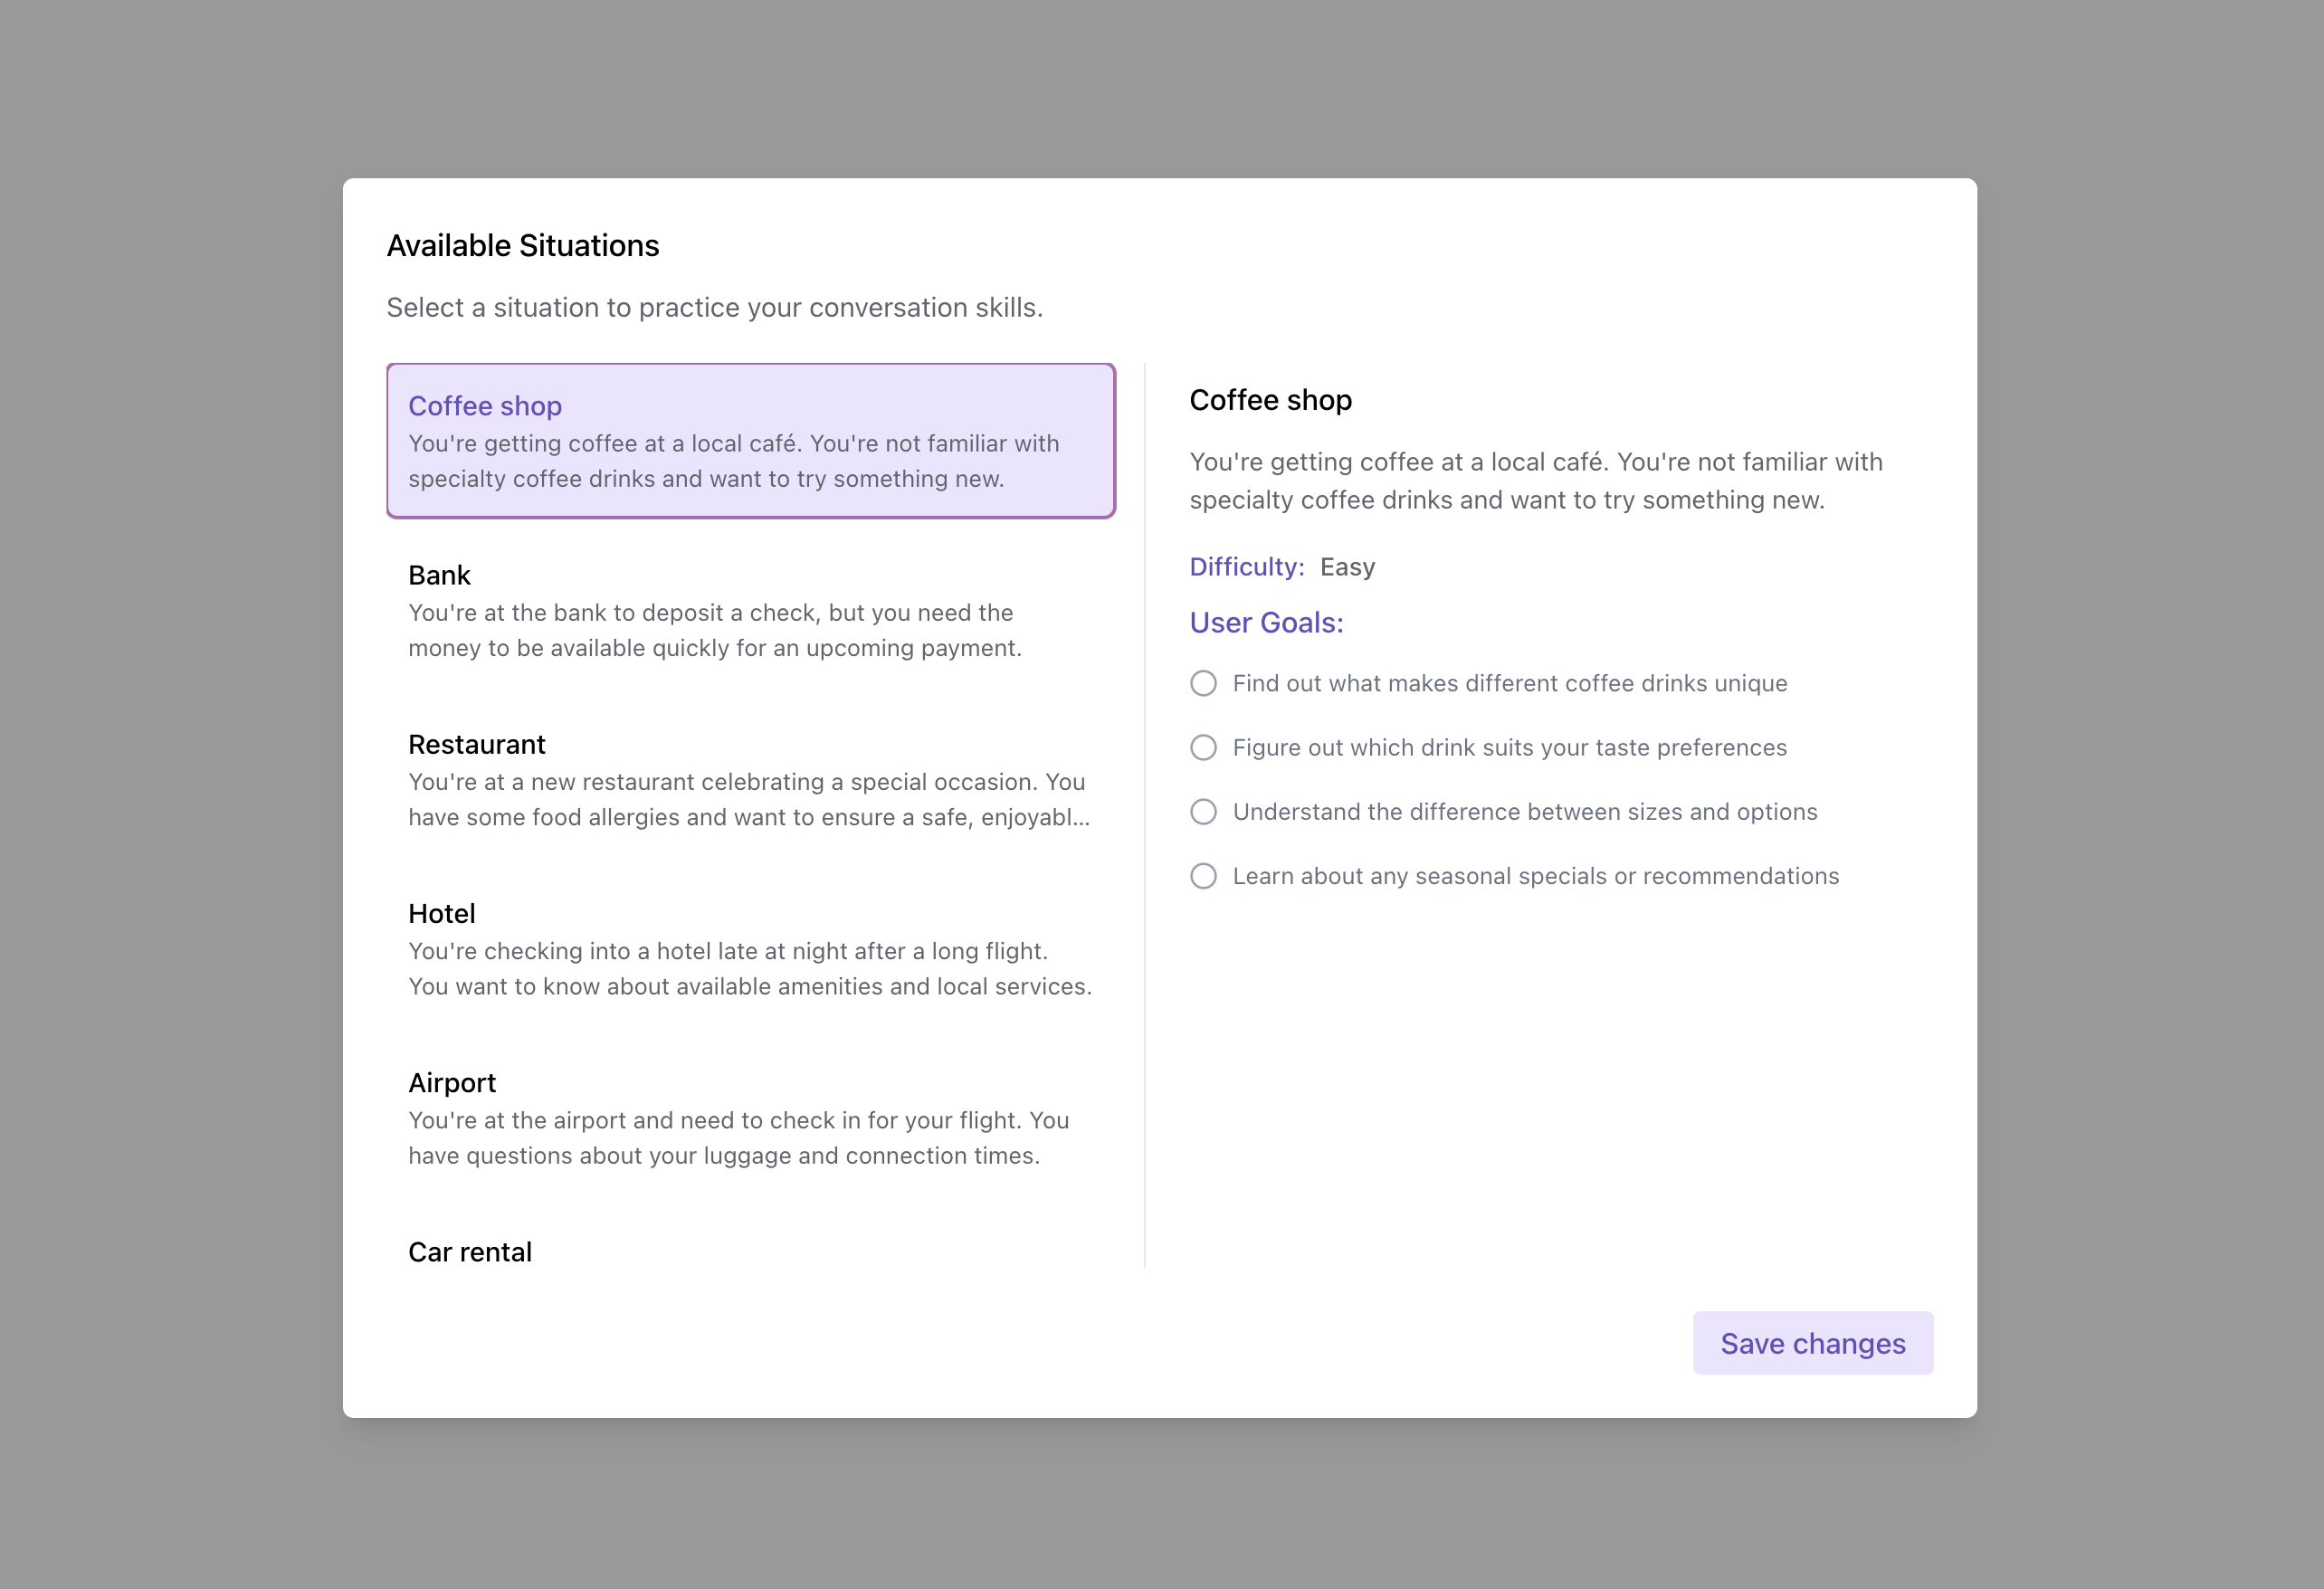
\includegraphics[width=0.8\textwidth]{figuras/screenshots/chat-complete.png}
    \caption{Sistema de diálogo mostrando una conversación de ejemplo}
    \label{fig:dialog-system}
\end{figure}

La Figura \ref{fig:dialog-system} ilustra el sistema de diálogo en funcionamiento, mostrando una conversación de ejemplo con el agente de aprendizaje. Los elementos destacables incluyen:

\begin{itemize}
    \item \textbf{Generación de respuestas contextuales:} El sistema proporciona respuestas adaptadas al contexto de la conversación y al nivel del estudiante, manteniendo coherencia temática y adecuación lingüística.
    
    \item \textbf{Integración de \gls{rag}:} Las respuestas se enriquecen con información recuperada de la base de conocimientos, proporcionando explicaciones precisas y ejemplos relevantes.
    
    \item \textbf{Sistema de corrección en tiempo real:} Feedback inmediato sobre errores gramaticales o léxicos, con explicaciones adaptadas al nivel del estudiante.
    
    \item \textbf{Indicadores de progreso:} Señales visuales que informan al estudiante sobre su avance en los objetivos de la conversación actual.
\end{itemize}

\subsection{Selector de Situaciones}
\label{selector-situaciones}

\begin{figure}[H]
    \centering
    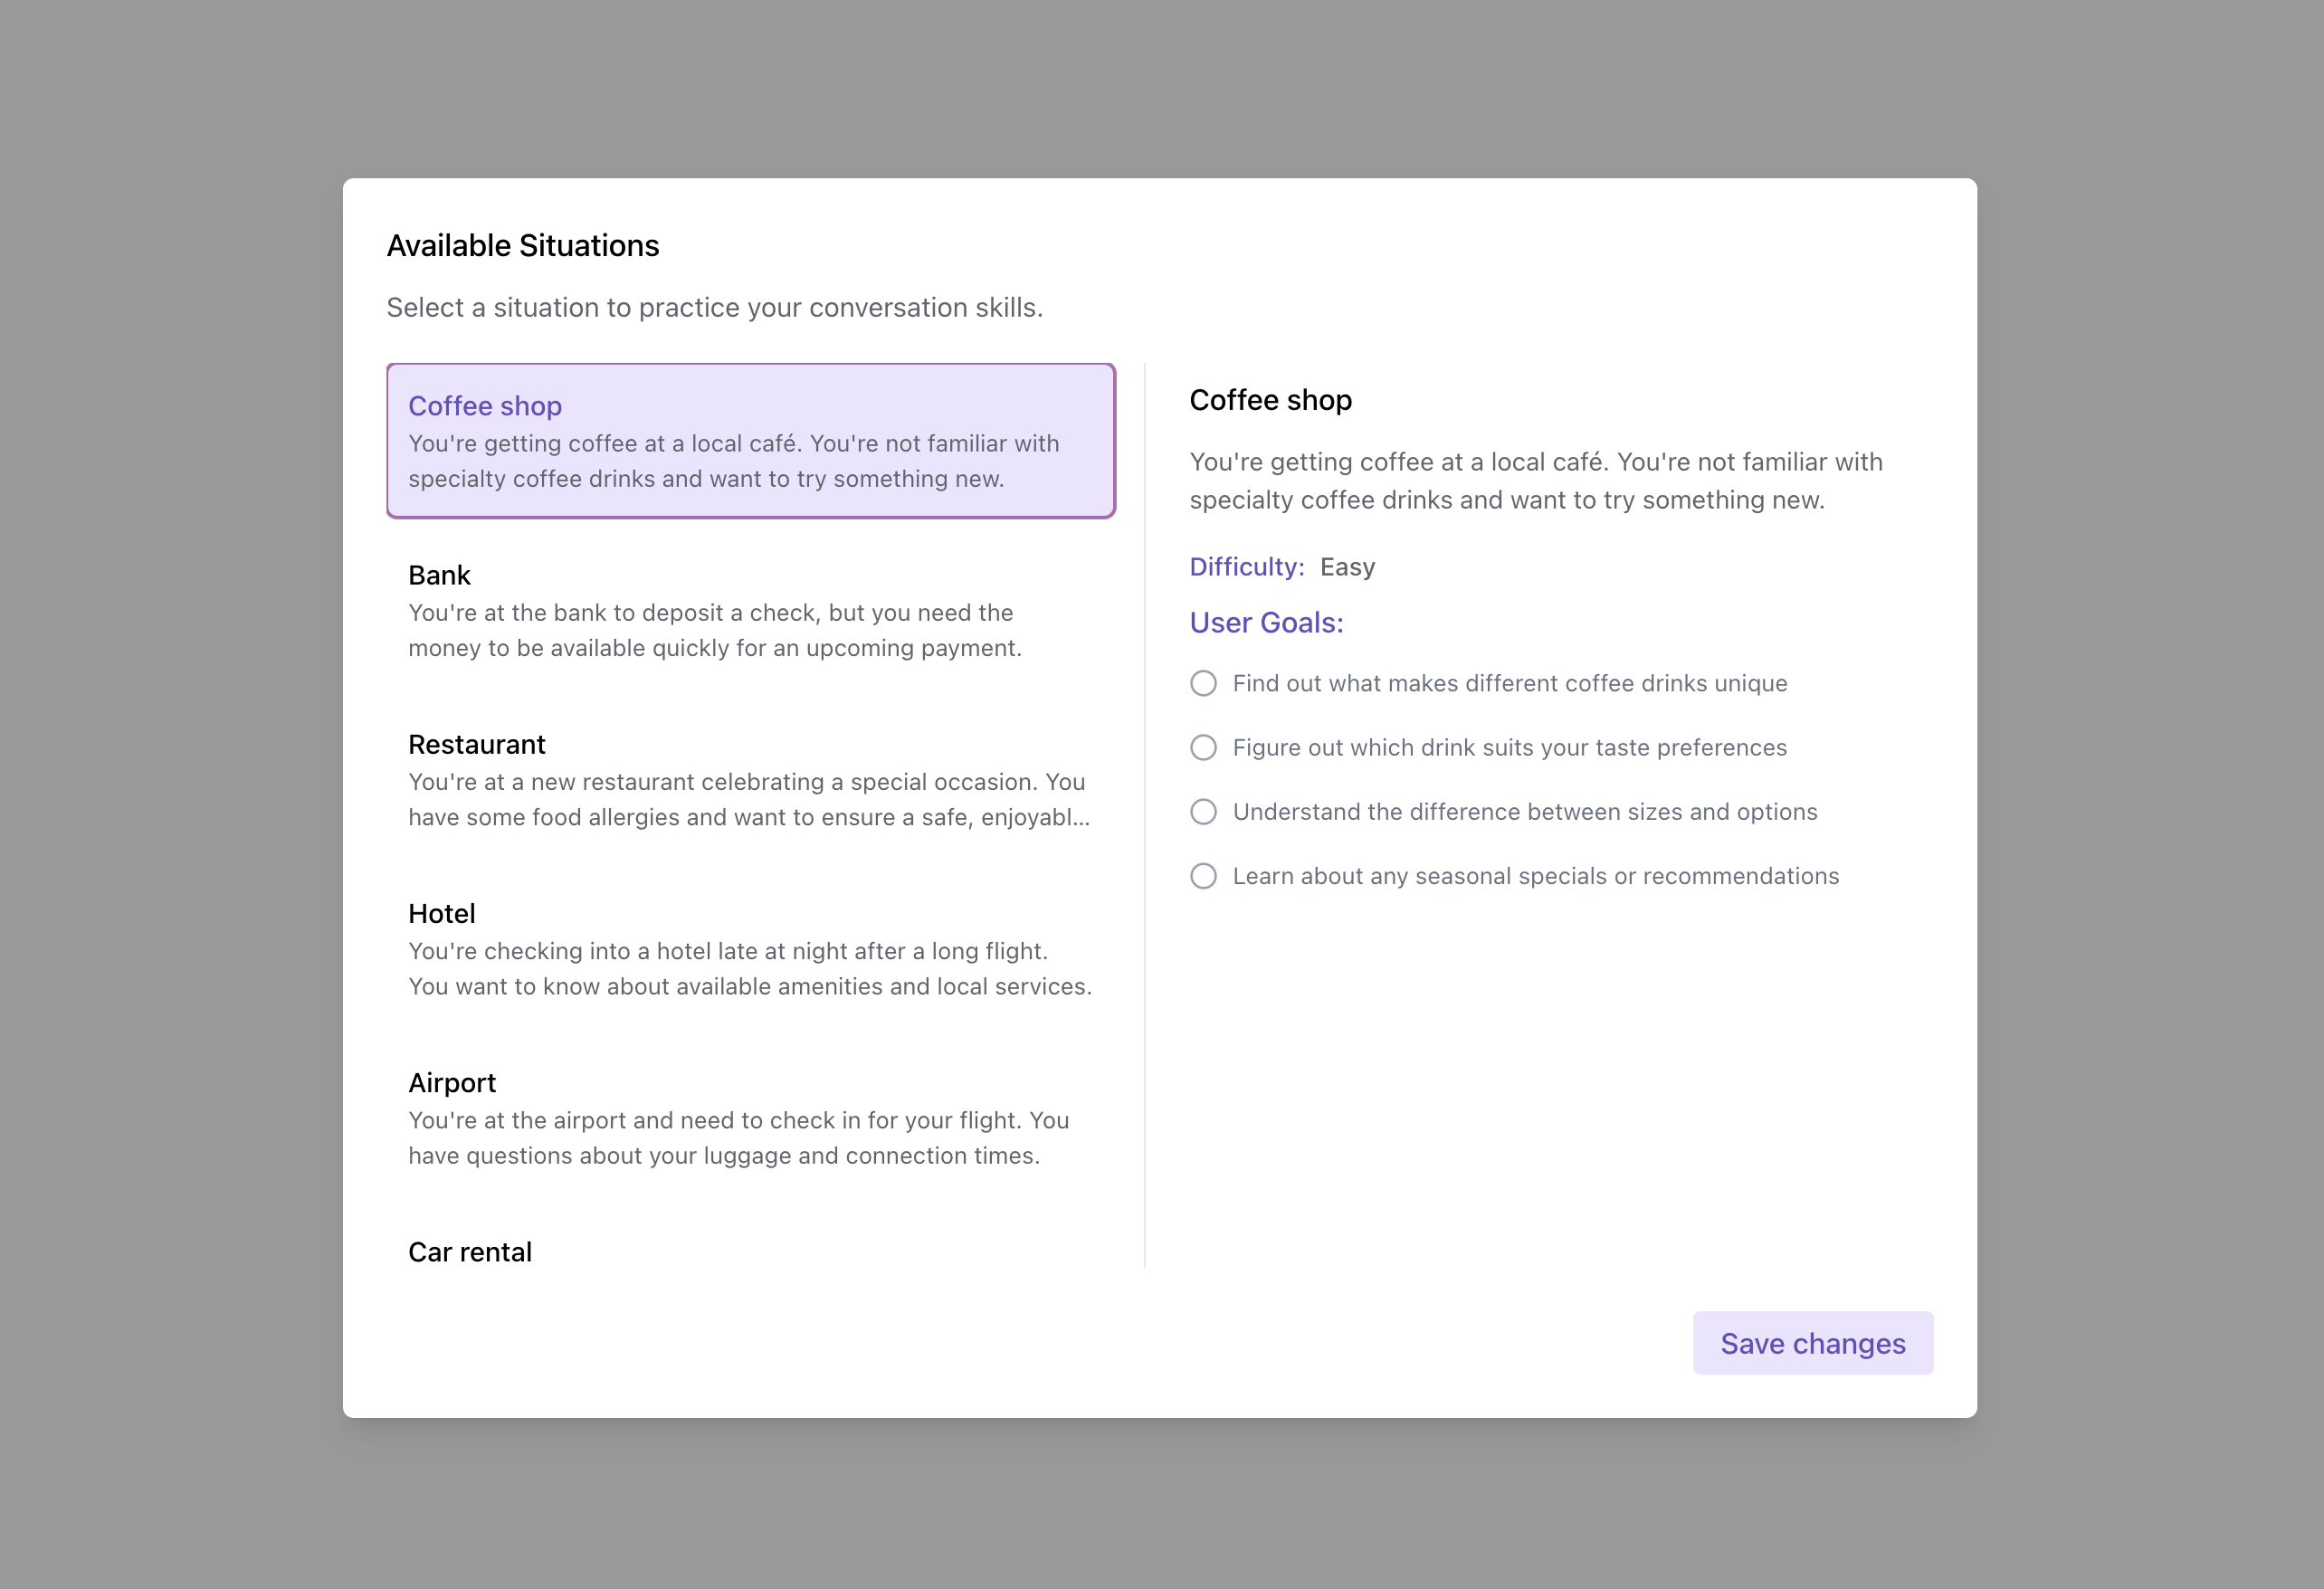
\includegraphics[width=0.8\textwidth]{figuras/screenshots/situation-picker.png}
    \caption{Interfaz de selección de contextos conversacionales y objetivos}
    \label{fig:situation-picker}
\end{figure}

La Figura \ref{fig:situation-picker} muestra la interfaz de selección de situaciones, un componente clave para la práctica contextualizada. Esta interfaz permite a los usuarios elegir escenarios específicos para su práctica conversacional, ofreciendo:

\begin{itemize}
    \item \textbf{Contextos Predefinidos:}
    \begin{itemize}
        \item Escenarios cotidianos como restaurantes, tiendas y oficinas
        \item Situaciones profesionales para entrevistas y reuniones
        \item Contextos académicos para estudiantes
        \item Situaciones sociales informales
    \end{itemize}
    
    \item \textbf{Sistema de Objetivos:}
    \begin{itemize}
        \item Lista clara de metas comunicativas a alcanzar durante la conversación
        \item Indicadores de progreso para cada objetivo específico
        \item Retroalimentación en tiempo real sobre el avance hacia las metas
    \end{itemize}
    
    \item \textbf{Personalización:}
    \begin{itemize}
        \item Adaptación automática del nivel de dificultad según el perfil del usuario
        \item Recomendaciones basadas en el historial de práctica y áreas de mejora
        \item Opciones para personalizar los objetivos específicos según necesidades
    \end{itemize}
\end{itemize}

\subsection{Panel de Análisis}
\label{panel-analisis}

\begin{figure}[H]
    \centering
    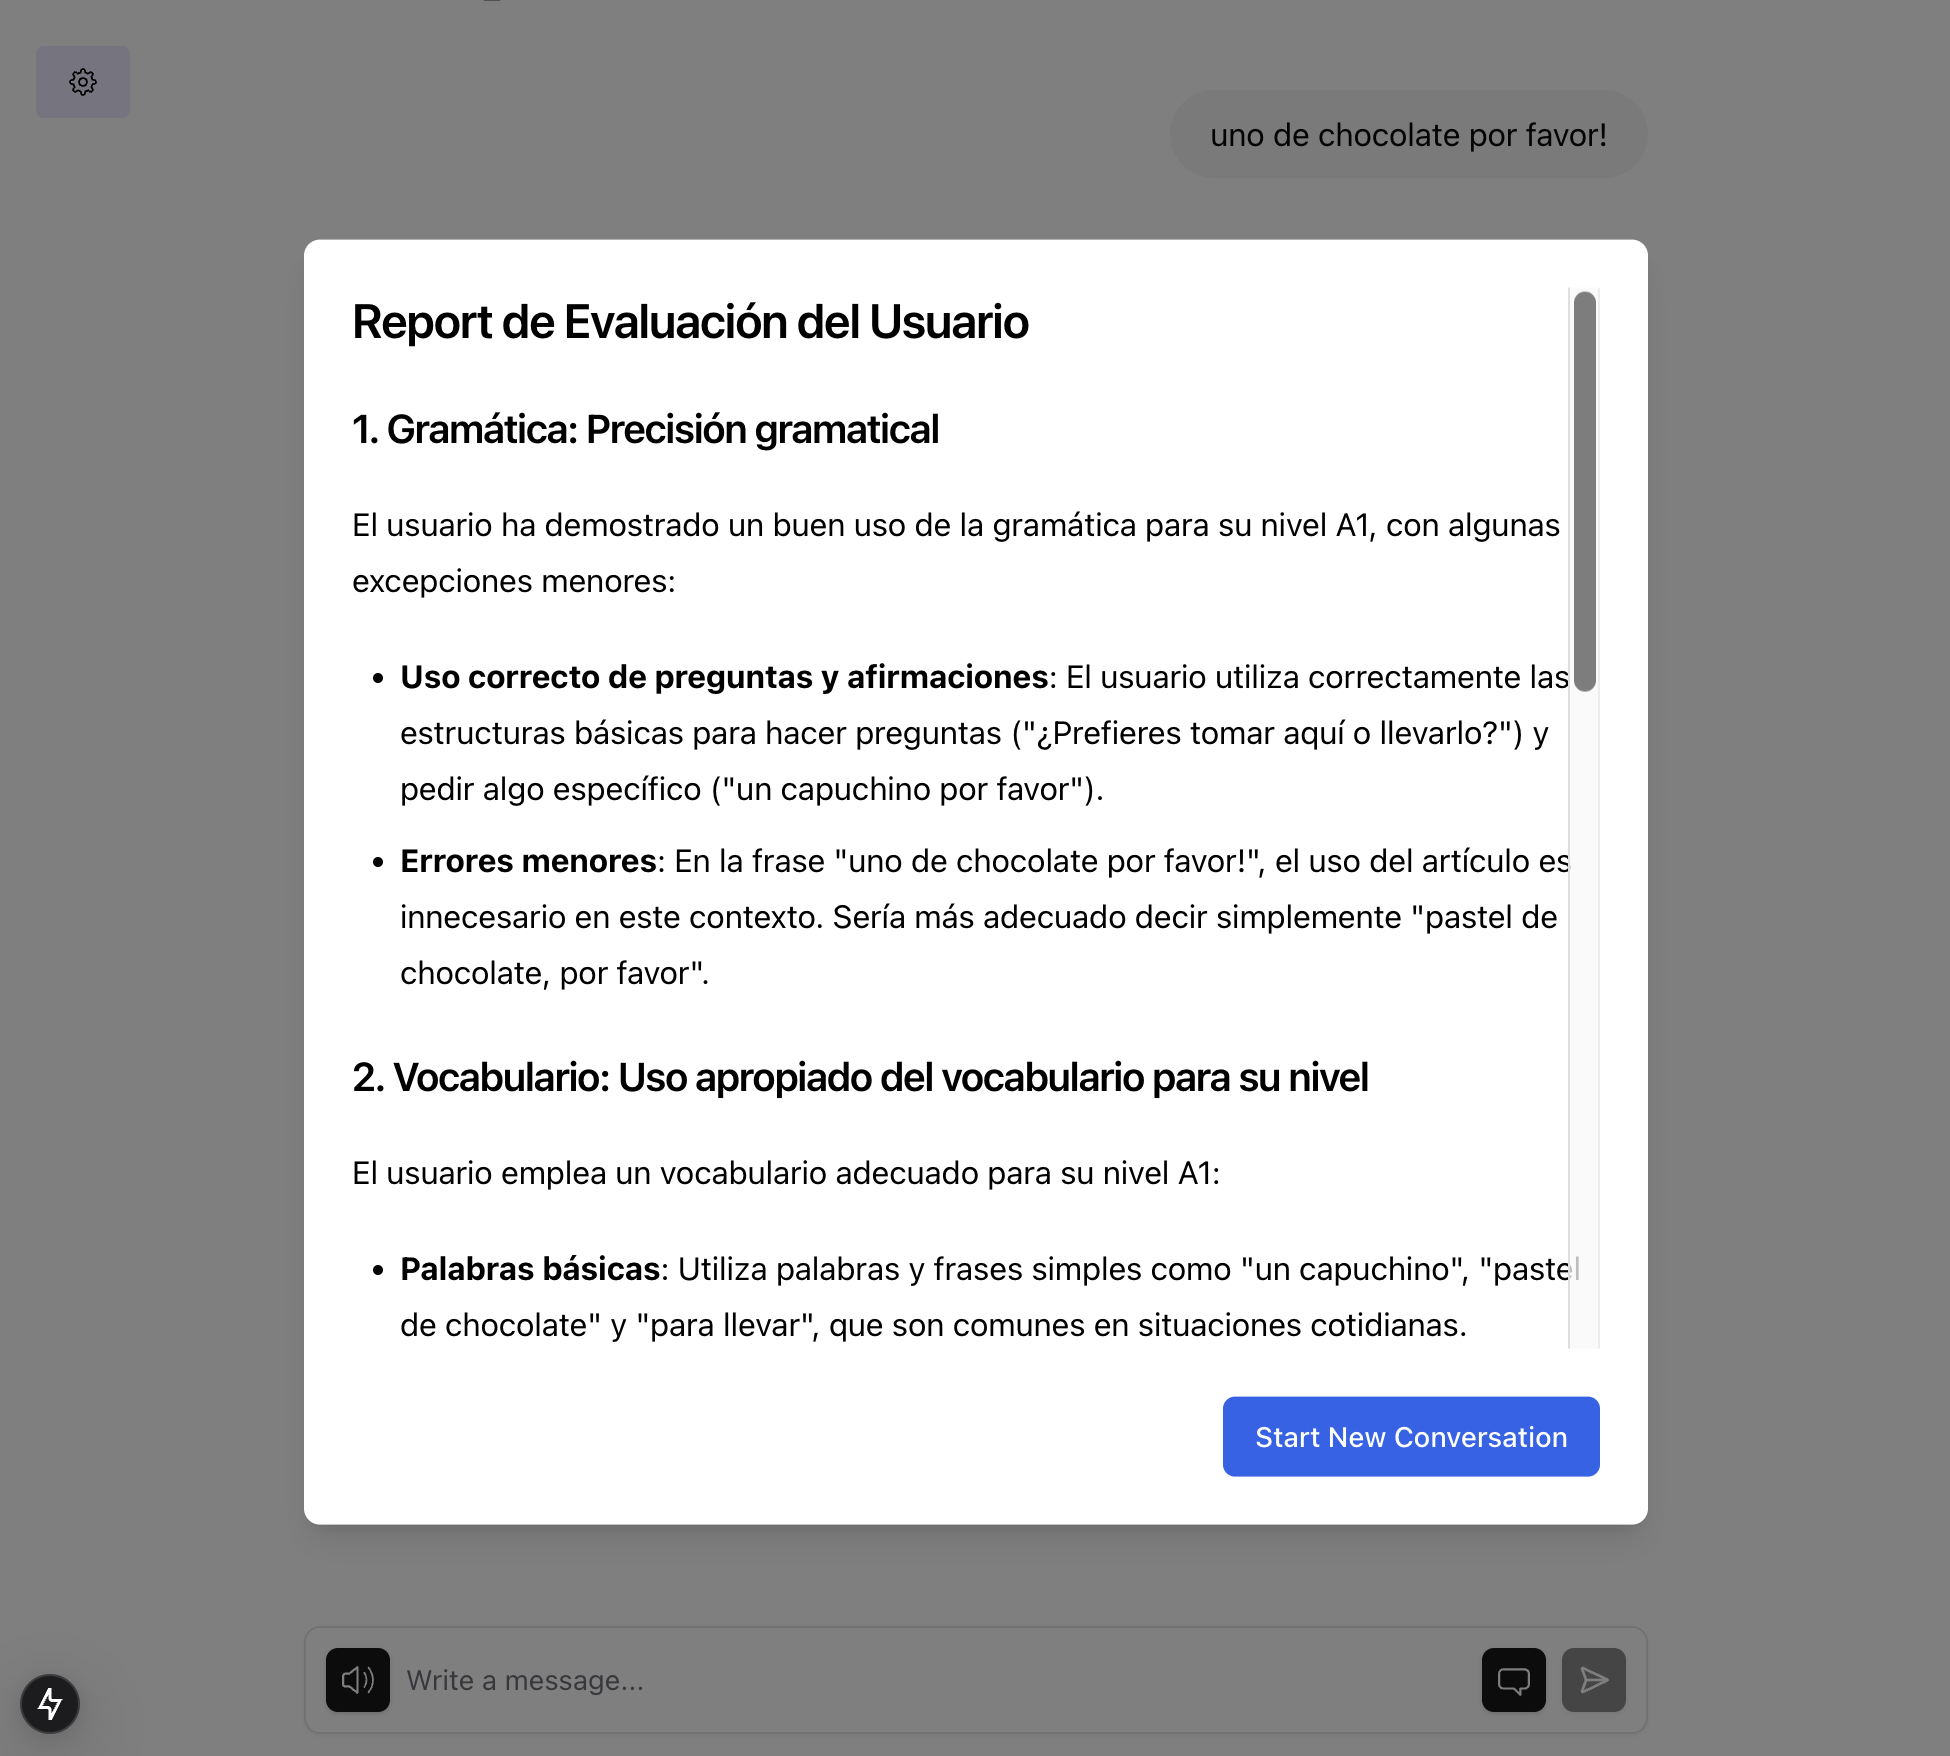
\includegraphics[width=0.8\textwidth]{figuras/screenshots/report.png}
    \caption{Panel de análisis mostrando métricas de aprendizaje}
    \label{fig:analytics-panel}
\end{figure}

La Figura \ref{fig:analytics-panel} muestra el panel de resultados, diseñado para proporcionar retroalimentación inmediata sobre el desempeño en la conversación. Este panel incluye:

\begin{itemize}
    \item \textbf{Objetivos cumplidos:} Registro de las metas alcanzadas durante la sesión de conversación.
    
    \item \textbf{Métricas de desempeño:} Evaluación de la conversación en tres dimensiones clave: gramática, vocabulario y fluidez, permitiendo al usuario identificar sus fortalezas y áreas de mejora.
    
    \item \textbf{Reporte personalizado:} Análisis detallado del desempeño con observaciones específicas sobre aspectos destacados y recomendaciones para mejorar.
    
    \item \textbf{Opciones de continuidad:} El usuario puede guardar su progreso y acceder posteriormente a la página de historial donde podrá visualizar su evolución a lo largo del tiempo.
\end{itemize}

\subsection{Visualización del Progreso de Aprendizaje}
\label{visualizacion-progreso}

\begin{figure}[H]
    \centering
    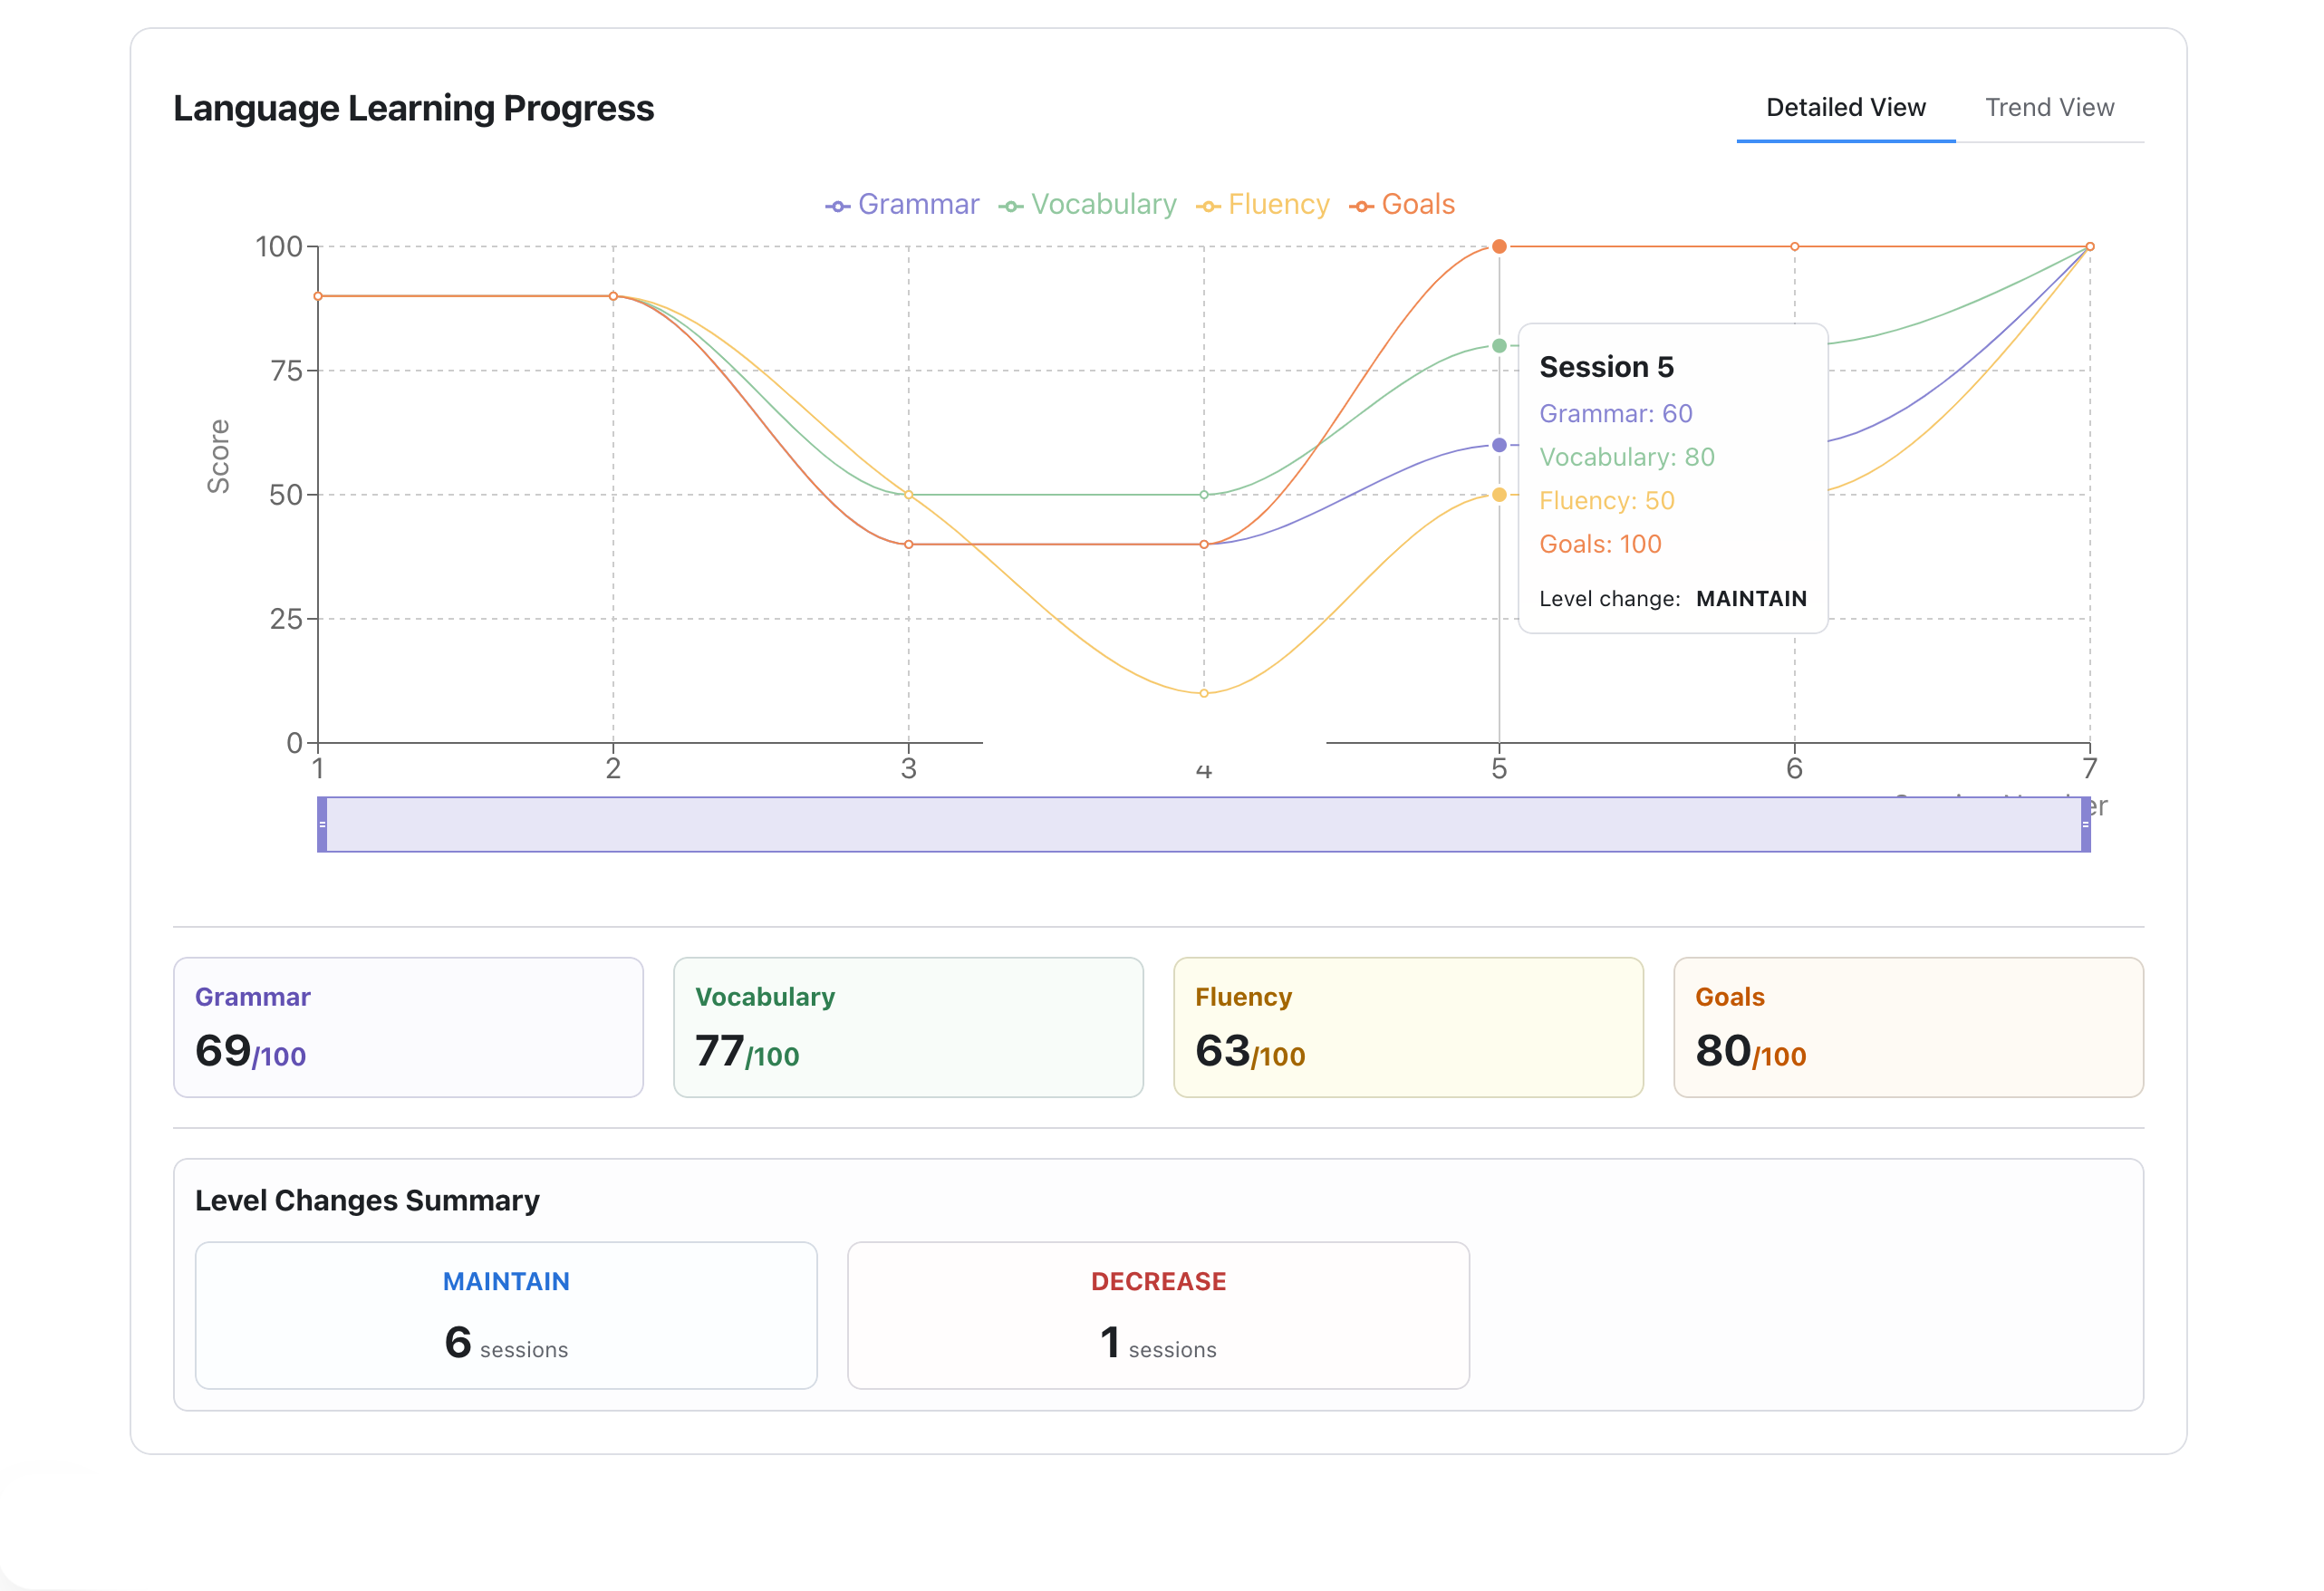
\includegraphics[width=0.8\textwidth]{figuras/screenshots/learning-history.png}
    \caption{Interfaz de visualización del progreso de aprendizaje con métricas detalladas}
    \label{fig:learning-history}
\end{figure}

La Figura \ref{fig:learning-history} muestra la interfaz de visualización del progreso de aprendizaje, un componente esencial para el seguimiento del desempeño del usuario. Esta herramienta proporciona una representación gráfica completa del desarrollo lingüístico a través de diversas funcionalidades integradas.

\begin{itemize}
    \item \textbf{Análisis Temporal Flexible:} Combina una vista detallada de sesiones individuales y una perspectiva de tendencias agrupadas, permitiendo al usuario alternar entre ambas modalidades para identificar tanto patrones generales como detalles específicos de su aprendizaje. El sistema incorpora controles interactivos que facilitan la exploración cronológica de los datos.
    
    \item \textbf{Evaluación Integral de Competencias Lingüísticas:} Monitoriza cuatro dimensiones fundamentales del aprendizaje: gramática, vocabulario, fluidez y cumplimiento de objetivos comunicativos. Cada métrica se presenta visualmente mediante un código de colores consistente que facilita la comparación entre habilidades y la identificación de fortalezas y áreas de mejora.
    
    \item \textbf{Análisis de Progresión de Nivel:} Ofrece un resumen visual de la trayectoria del aprendizaje, categorizando las sesiones según sus resultados (incremento, mantenimiento o descenso de nivel). Este componente proporciona contexto estadístico sobre el avance general, permitiendo correlacionar estrategias de práctica con resultados concretos.
    
    \item \textbf{Diseño Adaptativo y Accesible:} Implementado con Radix UI y técnicas responsivas para garantizar una experiencia óptima en cualquier dispositivo. La interfaz mantiene la integridad visual de los datos independientemente del tamaño de pantalla, priorizando la accesibilidad mediante contraste adecuado y elementos interactivos bien definidos.
\end{itemize}

Esta visualización del progreso constituye una herramienta fundamental para la reflexión metacognitiva del estudiante, permitiéndole identificar patrones en su aprendizaje y tomar decisiones informadas sobre sus futuras prácticas lingüísticas.

\section{Repositorios del Proyecto}
\label{sec:repositorios-proyecto}

El sistema ha sido desarrollado siguiendo una arquitectura cliente-servidor moderna, con separación clara entre la lógica de presentación y la de negocio. Todo el código fuente se encuentra disponible públicamente en GitHub bajo licencia MIT, promoviendo la transparencia, reproducibilidad y colaboración comunitaria.

\subsection{Estructura de Repositorios}
\label{subsec:estructura-repositorios}

\begin{itemize}
    \item \textbf{Frontend - Cliente:}
    \begin{itemize}
        \item Repositorio: \url{https://github.com/EmaSuriano/language-learning-client}
        \item Tecnologías: Next.js 14, TypeScript, Tailwind CSS
        \item Componentes principales:
              \begin{itemize}
                  \item Interfaz de chat basada en \gls{assistant-ui} con optimizaciones para aprendizaje
                  \item Selector de situaciones y objetivos con recomendaciones adaptativas
                  \item Gestión de estado con Zustand para manejo eficiente del contexto
                  \item Sistema de internacionalización con i18n (soporte para 8 idiomas)
                  \item Integración optimizada con API de audio para procesamiento de voz
              \end{itemize}
    \end{itemize}

    \item \textbf{Backend - Servidor:}
    \begin{itemize}
        \item Repositorio: \url{https://github.com/EmaSuriano/language-learning-server}
        \item Tecnologías: FastAPI, Python 3.10, LangChain, Stable-Baselines3
        \item Componentes principales:
              \begin{itemize}
                  \item Sistema \gls{rag} para recuperación contextual de recursos educativos
                  \item Integración con \gls{llm} (Phi-4) para generación de diálogos naturales
                  \item \gls{api-rest} con documentación OpenAPI para comunicación cliente-servidor
                  \item Implementación optimizada de Faster-Whisper y Kokoro-TTS
                  \item Sistema \gls{multi-agent} basado en LangChain para orquestación de agentes
                  \item Modelo \gls{ppo} implementado con Stable-Baselines3 para adaptación de nivel
              \end{itemize}
    \end{itemize}
\end{itemize}

\subsection{Documentación}
\label{subsec:documentacion-repositorios}

Ambos repositorios incluyen documentación exhaustiva para facilitar la comprensión, uso y extensión del sistema:

\begin{itemize}
    \item \textbf{Documentación General:}
    \begin{itemize}
        \item README principal con visión general del proyecto
        \item Guías de instalación detalladas para entornos de desarrollo y producción
        \item Diagramas de arquitectura y flujo de datos
        \item Guías de contribución para colaboradores externos
    \end{itemize}
    
    \item \textbf{Documentación Técnica:}
    \begin{itemize}
        \item Especificación completa de API mediante OpenAPI/Swagger
        \item Documentación de componentes y sus responsabilidades
        \item Variables de entorno requeridas con ejemplos y configuraciones recomendadas
        \item Guías de solución de problemas comunes
    \end{itemize}
    
    \item \textbf{Ejemplos y Tutoriales:}
    \begin{itemize}
        \item Ejemplos de uso para cada componente principal
        \item Tutoriales paso a paso para implementaciones personalizadas
        \item Guías para extensión de funcionalidades existentes
        \item Ejemplos de integración con sistemas externos
    \end{itemize}
\end{itemize}

Esta documentación exhaustiva facilita no solo la reproducibilidad de los resultados presentados, sino también la adaptación y extensión del sistema para diferentes contextos educativos y lingüísticos.

\section{Limitaciones Actuales y Trabajo Futuro}
\label{sec:limitaciones-trabajo-futuro}

A pesar de los resultados prometedores obtenidos, es importante reconocer las limitaciones actuales del sistema y definir las líneas de trabajo futuro para abordarlas.

\subsection{Limitaciones Identificadas}
\label{subsec:limitaciones-identificadas}

\begin{itemize}
    \item \textbf{Limitaciones Técnicas:}
    \begin{itemize}
        \item Precisión del sistema \gls{stt} insuficiente para acentos no nativos fuertes
        \item Tiempo de carga inicial del sistema relativamente alto (5-8 segundos)
        \item Dependencia de conexión a internet para funcionalidades avanzadas
        \item Consumo de recursos computacionales significativo para dispositivos de gama baja
    \end{itemize}

    \item \textbf{Limitaciones Pedagógicas:}
    \begin{itemize}
        \item Cobertura limitada de situaciones específicas de dominio (técnico, legal, médico)
        \item Sistema de evaluación aún no validado con metodologías educativas formales
        \item Adaptación insuficiente a diferentes estilos de aprendizaje
        \item Ausencia de mecanismos para aprendizaje colaborativo entre estudiantes
    \end{itemize}

    \item \textbf{Limitaciones de Validación:}
    \begin{itemize}
        \item Muestra reducida en pruebas preliminares (n=10)
        \item Período de evaluación relativamente corto (2 semanas)
        \item Ausencia de grupo de control para comparación con métodos tradicionales
        \item Falta de evaluación longitudinal del impacto en el aprendizaje
    \end{itemize}
\end{itemize}


\subsection{Trabajo Futuro}

En base a las limitaciones identificadas y los resultados preliminares, se plantean las siguientes líneas de trabajo futuro:

\begin{itemize}
    \item \textbf{Evaluación Exhaustiva:}
    \begin{itemize}
        \item Diseño de estudio con muestra ampliada (n>100) y diversificada geográficamente
        \item Implementación de evaluación longitudinal (3-6 meses) para medir impacto real
        \item Desarrollo de metodología comparativa con grupo de control usando métodos tradicionales
        \item Validación con profesionales de la enseñanza de idiomas y expertos en pedagogía
    \end{itemize}

    \item \textbf{Mejoras Técnicas:}
    \begin{itemize}
        \item Refinamiento del modelo \gls{ppo} mediante fine-tuning con datos reales de usuarios
        \item Adaptación específica del sistema \gls{stt} para mejorar precisión con acentos no nativos
        \item Optimización de la base de conocimientos del \gls{rag} con expansión temática y actualización automática
        \item Implementación de modos offline para funcionalidades básicas sin conexión
    \end{itemize}

    \item \textbf{Expansión de Funcionalidades:}
    \begin{itemize}
        \item Desarrollo de módulos específicos para dominios especializados (negocios, turismo, academia)
        \item Implementación de componente social para práctica colaborativa entre estudiantes
        \item Integración con contenido auténtico (noticias, videos, podcasts) para inmersión contextual
        \item Desarrollo de sistema de gamificación adaptativa para aumentar motivación y retención
    \end{itemize}
\end{itemize}

Estas líneas de trabajo futuro representan un plan estructurado para abordar las limitaciones actuales y expandir las capacidades del sistema, con el objetivo de maximizar su impacto educativo y mejorar la experiencia de aprendizaje para una gama más amplia de usuarios.

Los resultados presentados en este capítulo, aunque preliminares, proporcionan evidencia inicial sobre la viabilidad y potencial del enfoque propuesto. En el siguiente capítulo, se discutirán las conclusiones generales del trabajo, analizando las contribuciones realizadas, las lecciones aprendidas durante el desarrollo, y las implicaciones más amplias de estos avances para el futuro del aprendizaje de idiomas asistido por tecnología.